\documentclass[14pt]{extbook}
\usepackage{multicol, enumerate, enumitem, hyperref, color, soul, setspace, parskip, fancyhdr} %General Packages
\usepackage{amssymb, amsthm, amsmath, bbm, latexsym, units, mathtools} %Math Packages
\everymath{\displaystyle} %All math in Display Style
% Packages with additional options
\usepackage[headsep=0.5cm,headheight=12pt, left=1 in,right= 1 in,top= 1 in,bottom= 1 in]{geometry}
\usepackage[usenames,dvipsnames]{xcolor}
\usepackage{dashrule}  % Package to use the command below to create lines between items
\newcommand{\litem}[1]{\item#1\hspace*{-1cm}\rule{\textwidth}{0.4pt}}
\pagestyle{fancy}
\lhead{Makeup Progress Quiz 1}
\chead{}
\rhead{Version A}
\lfoot{6018-3080}
\cfoot{}
\rfoot{Spring 2021}
\begin{document}

\begin{enumerate}
\litem{
Write the equation of the line in the graph below in Standard form $Ax+By=C$. Then, choose the intervals that contain $A, B, \text{ and } C$.
\begin{center}
    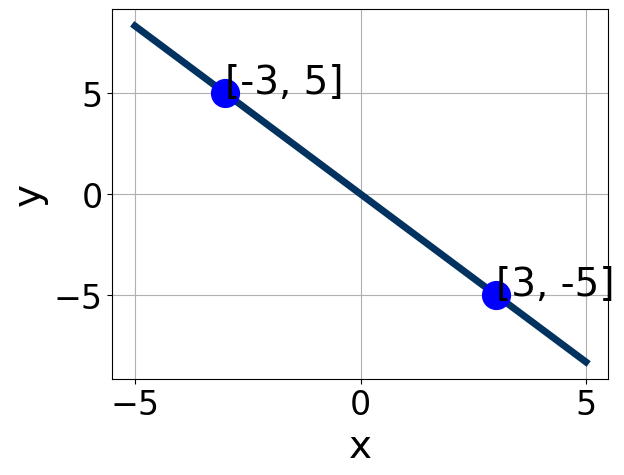
\includegraphics[width=0.5\textwidth]{../Figures/linearGraphToStandardCopyA.png}
\end{center}
\begin{enumerate}[label=\Alph*.]
\item \( A \in [-0.4, 4.7], \hspace{3mm} B \in [-1.29, -0.29], \text{ and } \hspace{3mm} C \in [-6, 5] \)
\item \( A \in [3.8, 7.3], \hspace{3mm} B \in [-3.62, -2.66], \text{ and } \hspace{3mm} C \in [-6, 5] \)
\item \( A \in [3.8, 7.3], \hspace{3mm} B \in [1.99, 3.57], \text{ and } \hspace{3mm} C \in [-6, 5] \)
\item \( A \in [-0.4, 4.7], \hspace{3mm} B \in [-0.69, 1.75], \text{ and } \hspace{3mm} C \in [-6, 5] \)
\item \( A \in [-5.4, -3.5], \hspace{3mm} B \in [-3.62, -2.66], \text{ and } \hspace{3mm} C \in [-6, 5] \)

\end{enumerate} }
\litem{
Solve the linear equation below. Then, choose the interval that contains the solution.\[ \frac{-7x + 8}{5} - \frac{6x -9}{7} = \frac{-3x -4}{2} \]\begin{enumerate}[label=\Alph*.]
\item \( x \in [27.6, 29.2] \)
\item \( x \in [2.6, 3.3] \)
\item \( x \in [-0.6, 2.4] \)
\item \( x \in [5.5, 7.1] \)
\item \( \text{There are no real solutions.} \)

\end{enumerate} }
\litem{
Solve the equation below. Then, choose the interval that contains the solution.\[ -4(-5x -8) = -13(-15x + 9) \]\begin{enumerate}[label=\Alph*.]
\item \( x \in [0.44, 0.69] \)
\item \( x \in [0.8, 0.94] \)
\item \( x \in [-0.76, -0.33] \)
\item \( x \in [0.38, 0.43] \)
\item \( \text{There are no real solutions.} \)

\end{enumerate} }
\litem{
Find the equation of the line described below. Write the linear equation as $ y=mx+b $ and choose the intervals that contain $m$ and $b$.\[ \text{Perpendicular to } 8 x + 3 y = 13 \text{ and passing through the point } (10, 3). \]\begin{enumerate}[label=\Alph*.]
\item \( m \in [0.11, 0.57] \hspace*{3mm} b \in [-10, -3] \)
\item \( m \in [2.04, 2.72] \hspace*{3mm} b \in [-1.75, 0.25] \)
\item \( m \in [0.11, 0.57] \hspace*{3mm} b \in [-1.75, 0.25] \)
\item \( m \in [-2.04, -0.06] \hspace*{3mm} b \in [4.75, 14.75] \)
\item \( m \in [0.11, 0.57] \hspace*{3mm} b \in [-0.25, 3.75] \)

\end{enumerate} }
\litem{
Write the equation of the line in the graph below in Standard form $Ax+By=C$. Then, choose the intervals that contain $A, B, \text{ and } C$.
\begin{center}
    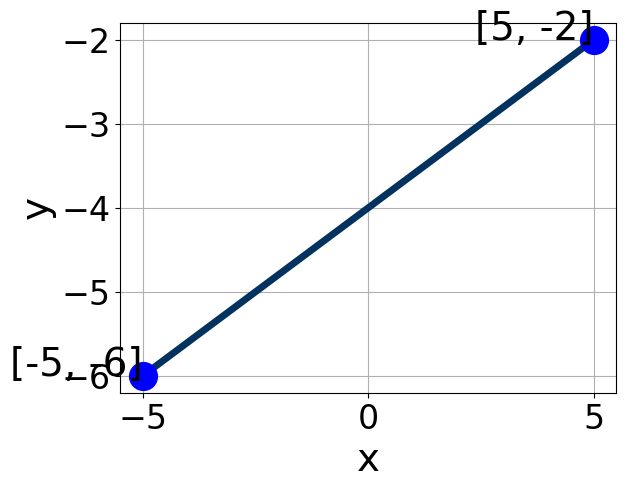
\includegraphics[width=0.5\textwidth]{../Figures/linearGraphToStandardA.png}
\end{center}
\begin{enumerate}[label=\Alph*.]
\item \( A \in [-3.7, -0.9], \hspace{3mm} B \in [3.6, 6.3], \text{ and } \hspace{3mm} C \in [-21, -17] \)
\item \( A \in [-1.8, 1.6], \hspace{3mm} B \in [-4.2, 0.5], \text{ and } \hspace{3mm} C \in [0, 5] \)
\item \( A \in [-1.8, 1.6], \hspace{3mm} B \in [0.2, 3.1], \text{ and } \hspace{3mm} C \in [-5, 0] \)
\item \( A \in [1.3, 4.9], \hspace{3mm} B \in [-6.1, -3.4], \text{ and } \hspace{3mm} C \in [17, 29] \)
\item \( A \in [1.3, 4.9], \hspace{3mm} B \in [3.6, 6.3], \text{ and } \hspace{3mm} C \in [-21, -17] \)

\end{enumerate} }
\litem{
First, find the equation of the line containing the two points below. Then, write the equation as $ y=mx+b $ and choose the intervals that contain $m$ and $b$.\[ (-7, 9) \text{ and } (9, -4) \]\begin{enumerate}[label=\Alph*.]
\item \( m \in [-0.19, 1.81] \hspace*{3mm} b \in [-12.2, -10.4] \)
\item \( m \in [-3.81, 0.19] \hspace*{3mm} b \in [-3.9, -2.7] \)
\item \( m \in [-3.81, 0.19] \hspace*{3mm} b \in [1.4, 5.1] \)
\item \( m \in [-3.81, 0.19] \hspace*{3mm} b \in [-14.2, -12.1] \)
\item \( m \in [-3.81, 0.19] \hspace*{3mm} b \in [15.6, 17] \)

\end{enumerate} }
\litem{
Solve the linear equation below. Then, choose the interval that contains the solution.\[ \frac{-5x + 8}{2} - \frac{-8x + 5}{5} = \frac{-4x + 5}{3} \]\begin{enumerate}[label=\Alph*.]
\item \( x \in [-8.5, -7.3] \)
\item \( x \in [-0.5, 1.3] \)
\item \( x \in [-3.2, -2.8] \)
\item \( x \in [3.7, 4.9] \)
\item \( \text{There are no real solutions.} \)

\end{enumerate} }
\litem{
Solve the equation below. Then, choose the interval that contains the solution.\[ -18(-8x + 15) = -7(17x -13) \]\begin{enumerate}[label=\Alph*.]
\item \( x \in [-1.22, 0.49] \)
\item \( x \in [-0.58, 1.32] \)
\item \( x \in [6.88, 7.35] \)
\item \( x \in [1.27, 1.54] \)
\item \( \text{There are no real solutions.} \)

\end{enumerate} }
\litem{
Find the equation of the line described below. Write the linear equation as $ y=mx+b $ and choose the intervals that contain $m$ and $b$.\[ \text{Perpendicular to } 8 x - 3 y = 13 \text{ and passing through the point } (-9, 6). \]\begin{enumerate}[label=\Alph*.]
\item \( m \in [-1.3, 0.04] \hspace*{3mm} b \in [1.62, 3.62] \)
\item \( m \in [-0.32, 1.74] \hspace*{3mm} b \in [5.38, 10.38] \)
\item \( m \in [-1.3, 0.04] \hspace*{3mm} b \in [-5.62, 2.38] \)
\item \( m \in [-3.4, -2.39] \hspace*{3mm} b \in [1.62, 3.62] \)
\item \( m \in [-1.3, 0.04] \hspace*{3mm} b \in [15, 18] \)

\end{enumerate} }
\litem{
First, find the equation of the line containing the two points below. Then, write the equation as $ y=mx+b $ and choose the intervals that contain $m$ and $b$.\[ (3, 3) \text{ and } (7, 2) \]\begin{enumerate}[label=\Alph*.]
\item \( m \in [-0.1, 0.48] \hspace*{3mm} b \in [0.21, 0.77] \)
\item \( m \in [-0.54, -0.12] \hspace*{3mm} b \in [3.1, 4.78] \)
\item \( m \in [-0.54, -0.12] \hspace*{3mm} b \in [-5.69, -4.83] \)
\item \( m \in [-0.54, -0.12] \hspace*{3mm} b \in [-0.76, 0.02] \)
\item \( m \in [-0.54, -0.12] \hspace*{3mm} b \in [-4.21, -3.38] \)

\end{enumerate} }
\end{enumerate}

\end{document}